\documentclass[12pt]{beamer}
\usepackage[T2A]{fontenc} 
\usepackage[utf8]{inputenc} 
\usepackage{algorithm}
\usepackage{algorithmic}
\usepackage{makecell}
\usepackage[english, ukrainian]{babel} 
\mode<presentation>{
	\usetheme{CambridgeUS}
    \setbeamercovered{transparent}
}
%% preamble
\title{Реалізація алгоритму розв'язування
	інтегральних рівнянь та задачі Діріхле для
	рівняння Лапласа використовуючи ієрархічні
	матриці}
\author{Солук Олена}
\date[ 2019]
{\large{Львівський національний університет імені І.Франка}}
\begin{document}
\begin{frame}
	\titlepage
\end{frame}
%% normal frame
\begin{frame}{Кластерне дерево}
	\begin{block}{}
		$$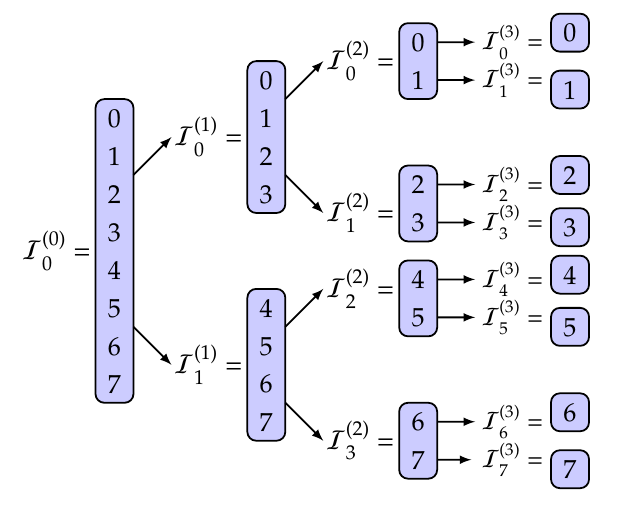
\includegraphics[scale=0.48]{1_0}$$
	\end{block}
\end{frame}
\begin{frame}
\frametitle{Блочне кластерне дерево}
	\begin{block}{Означення}
	Нехай $\mathbb{T}_{I}$ і $\mathbb{T}_{J}$ - кластерні дерева над множинами індексів $I$ та $J$ відповідно. Кластерне дерево $\mathbb{T}_{I\times J}=\mathbb{T}_{\mathbb{T}_{I}\times \mathbb{T}_{J}}=(V,E)$ називається блочним кластерним деревом над добутком множини індексів $I\times J$, якщо $\forall v\in V$ виконуються наступні умови:
		\begin{enumerate}
			\item[-] $\mathbb{T}^{(0)}_{I\times J}=I\times J$
			\item[-] Якщо $v\in \mathbb{T}^{(l)}_{I\times J}$, то існують $\tau \in \mathbb{T}^{(l)}_I$ i $\sigma \in \mathbb{T}^{(l)}_J$ такі, що $v=\tau \times \sigma$.
			\item[-] Для синів $v=\tau \times \sigma$, де  $\tau \in \mathbb{T}_I$ i $\sigma \in \mathbb{T}_J$ виконується
			\newline
			S(v)=$\begin{cases}
			$\O,$\text{якщо $S(\tau)=\O$ або $S(\sigma)=\O$}\\
			$$\{\tau^{\prime}\times\sigma^{\prime} : \tau^{\prime} \in S(\tau),\sigma^{\prime} \in S(\sigma)\}$,$\text{інакше}
			\end{cases}$
		\end{enumerate}
	\end{block}
\end{frame}

\begin{frame}{Приклад побудови блочного кластерного дерева}
	\begin{block}{}
		\centering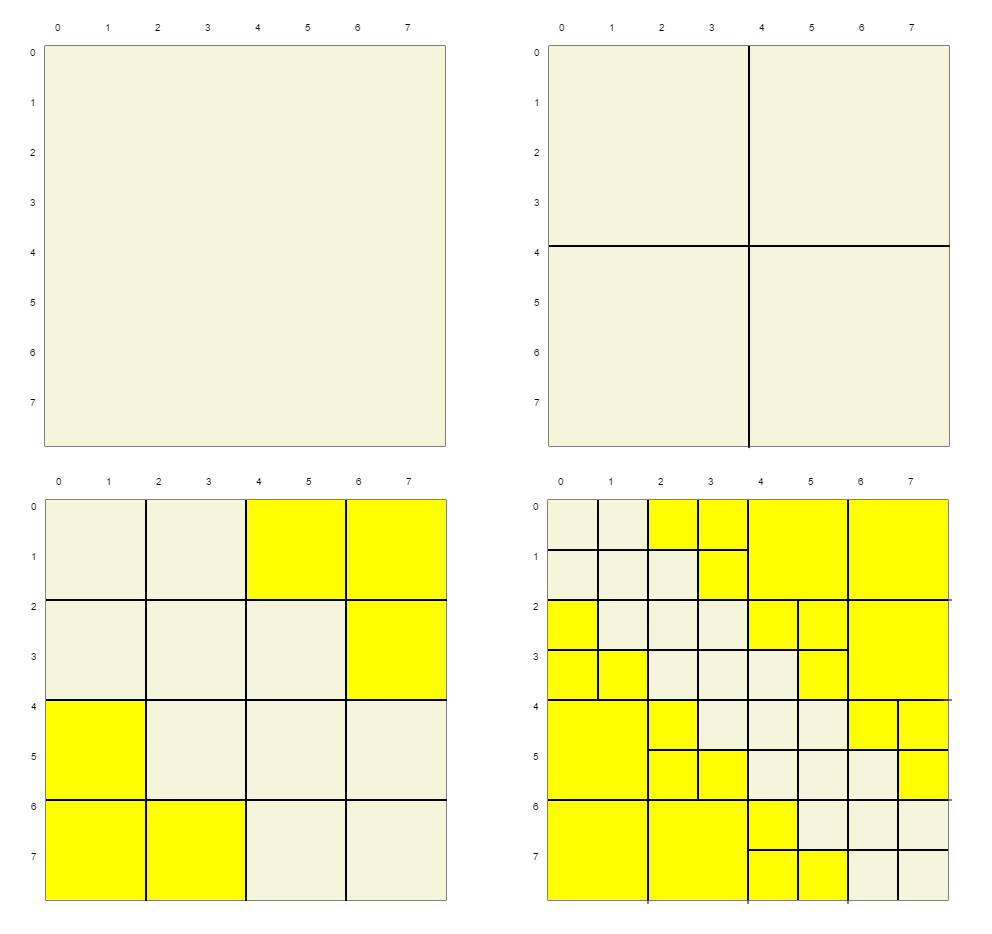
\includegraphics[scale=0.27]{1_3}
	\end{block}
\end{frame}
\begin{frame}
\frametitle{Означення $\mathcal{H}$-матриці}
	\begin{block}{Означення}
		Нехай $\mathbb{T}_{I\times I}$ - блочне кластерне дерево над множиною індексів $I$. Означаємо множину $\mathcal{H}$-матриць як
			$$\mathcal{H}(\mathbb{T}_{I\times I},m):=\{M\in\mathbb{R}^{I\times I}|rank(M|_{t\times s})\le m \text{ для всіх}$$ $$\text{допустимих листків } t\times s \text{ дерева } \mathbb{T}_{I\times I} \}$$
	\end{block}
	\begin{block}{}
	
		\begin{columns}[onlytextwidth,T]
			\begin{column}{.55\linewidth}
				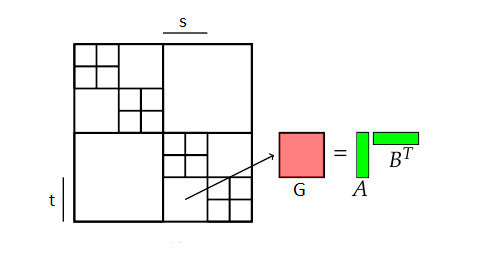
\includegraphics[width=\linewidth]{1_6}
			\end{column}
			\begin{column}{.48\linewidth}
				\vspace*{1cm}
				$G|_{t\times s}=AB^\top,$\\ $A\in\mathbb{R}^{t\times\{0,\dots,m-1\}},$\\ $B\in\mathbb{R}^{s\times\{0,\dots,m-1\}}$
			\end{column}
		\end{columns}
	\end{block}
\end{frame}
\begin{frame}{Внутрішня задача Діріхле  для рівняння Лапласа }
	\begin{block}{}
		$\Omega\subset\mathbb{R}^2$ - обмежена однозв'язна область з границею $\Gamma\subset C^2$, $f\in C(\Gamma)$ - задана.
		Знайти $u\in C^2(\Omega)\cap C(\bar{\Omega}):$
		$$\triangle u=0 \text{ в }\Omega\eqno(1)$$
		$$u=f\text{ на }\Gamma\eqno(2)$$
	\end{block}
	\begin{block}{}
	$$\Upsilon_{slp}[u](x):=-\frac{1}{2\pi}\int_{\Gamma}\log(\|x-y\|)u(y)dy\eqno(3)$$
	$$a_{slp}(u,v):=-\frac{1}{2\pi}\int_{\Gamma}v(x)\int_{\Gamma}\log(\|x-y\|)u(y)dydx\eqno(4)$$
		
	\end{block}
\end{frame}
\begin{frame}{Область і базисні функції}
	\begin{block}{}
	\begin{columns}[onlytextwidth,T]
		\begin{column}{.45\linewidth}
			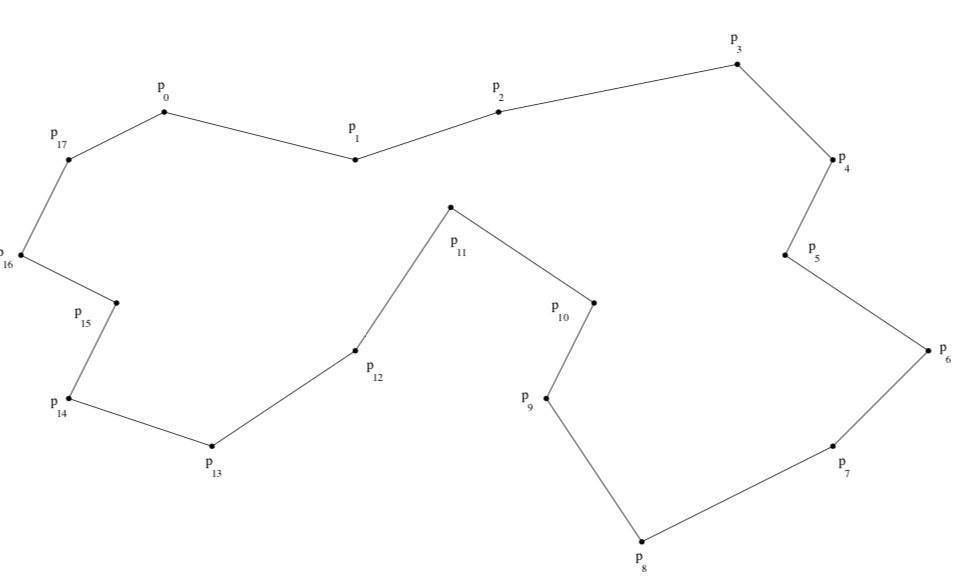
\includegraphics[width=\linewidth]{2_2}
		\end{column}
		\begin{column}{.55\linewidth}

			$$\gamma_i:[0,1]\rightarrow\mathbb{R}^2$$
			$$y\mapsto p_{i-1}(1-y)+p_iy$$
			\begin{equation*}
			\varphi_i(x)=\begin{cases}
			1,\quad\text{якщо $ x\in \gamma_i[0,1]$}\\
			0,\quad\text{якщо $ x\not\in \gamma_i[0,1]$}
			\end{cases}
			\end{equation*}
		\end{column}
	\end{columns}
	\end{block}
	\begin{block}{}
	$$G_{ij}=-\frac{1}{2\pi}\int_{\Gamma}\varphi_i(x)\int_{\Gamma}\log(\|x-y\|)\varphi_j(y)dydx\eqno(5)$$
	$$=-\frac{1}{2\pi}\|p_i-p_{i-1}\| \|p_j-p_{j-1}\|\int_{0}^{1}\int_{0}^{1}\log(\|\gamma_i(x)-\gamma_j(y)\|)dydx\eqno(6)$$
	\end{block}
\end{frame}
\begin{frame}{Геометрична бісекція і обмежувальні коробки}
	
		$$i\in I, \Omega_i:=supp(\varphi_i),x_i \in\Omega_i$$
		 $\hat t\in I$ - множина індексів, що відповідає кластеру $t$
		$$a_l:=\min \{(x_i)_l : i\in \hat t\}$$
		$$b_l:=\max \{(x_i)_l : i\in \hat t\}$$
		для кожного $l\in \{1,...,d\}$. \\
		$Q_t =[a_1,b_1]\times...\times[a_d,b_d]$ - обмежувальна коробка.
		$$min(diam(\Omega_{\tau}),diam(\Omega_{\sigma}))\le \eta\cdot dist(\Omega_{\tau},\Omega_{\sigma})\eqno(7)$$
		$$max(diam(Q_{t}),diam(Q_{s}))\le \eta\cdot dist(Q_{t},Q_{s})\eqno(8)$$
\end{frame}

\begin{frame}{Інтерполяція}
	
		$$\tilde{g}(x,y):=\sum_{v\in K}g(x_v,y)\mathcal{L}_v(x)\eqno(9)$$
		
		$$\tilde{G}_{ij}=\int_{\Omega}\varphi_i(x)\int_{\Omega}\tilde{g}(x,y)\varphi_j(y)dy dx = $$$$\sum_{v\in K}\int_{\Omega}\varphi_i(x)\mathcal{L}_v(x)dx\int_{\Omega}\varphi_j(y)g(x_v,y)dy=(AB^\top)_{ij}\eqno(10)$$
		
		Якщо $diam(Q_t)\le diam(Q_s)$
			$$A_{iv}^{t,s}=\int_{\Omega}\varphi_i(x)\mathcal{L}_v^t(x)dx\;\;\;\;\;\;\;\;\;\;\;\;\;\;\;
		B_{jv}^{t,s}=\int_{\Omega}\varphi_j(y)g(x_v^t,y)dy$$
		інакше
		$$A_{iv}^{t,s}=\int_{\Omega}\varphi_i(x)g(x,x_v^s)dx
		\;\;\;\;\;\;\;\;\;\;\;\;\;\;\;B_{jv}^{t,s}=\int_{\Omega}\varphi_j(y)\mathcal{L}_v^s(y)dy$$
		
\end{frame}

\begin{frame}{Інтерполяція}
	$$K:=\{v\in\mathbb{N}_0^d:v_i\le m \mbox{ для всіх } i\in \{1,...,d\}\}$$
	
	$$(x_v)_{v=0}^m=\left(cos\left(\frac{2v+1}{2m+2}\pi\right)\right)_{v=0}^m\;\;\;\;\; \mathcal{L}_v(x)=\prod_{\mu=0,\mu\not=v}^{m}\frac{x-x_\mu}{x_v-x_\mu}\eqno(11)$$
	
	$$\mathcal{L}_v^t(x)=\prod_{i=1}^{d}\mathcal{L}_{v_i}^{[a_i,b_i]}(x_i)=\prod_{i=1}^{d}\prod_{\mu=0,\mu\not=v_i}^{m}\frac{x_i-x_\mu^{[a_i,b_i]}}{x_{v_i}^{[a_i,b_i]}-x_\mu^{[a_i,b_i]}}\eqno(12)$$
	
	$$A_{iv}^{(t,s)}=\|p_i-p_{i-1}\|\int_{0}^{1}\mathcal{L}_v^t(\gamma_i(x))dx$$
	$$B_{jv}^{t,s}=-\frac{1}{2\pi}\|p_j-p_{j-1}\|\int_{0}^{1}\log(\|x_v^t-\gamma_j(y)\|)dy$$ 
\end{frame}

\begin{frame}{Чисельні експерименти}
	Розглядаємо рівняння
	$$f(x)=\log\|x-x^*\|$$ 
	на $D = (\cos(t+10), \sin(t)), x^*\not \in D, x^*=(2,2)$.
	\begin{center}
		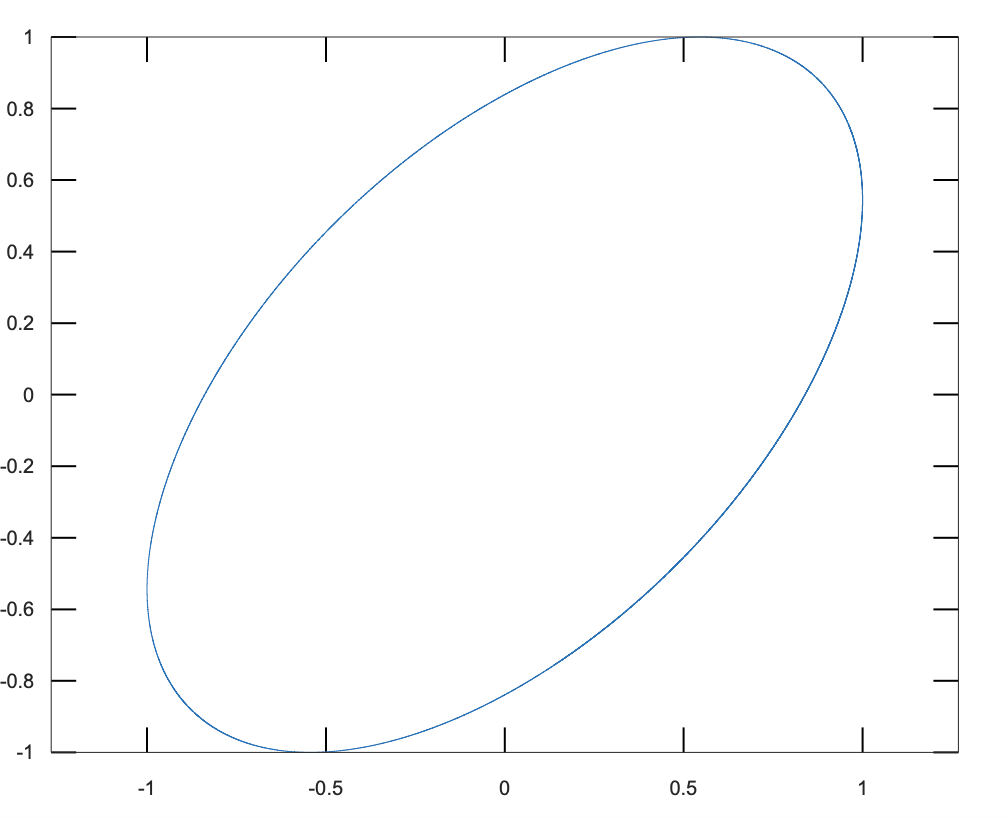
\includegraphics[scale=0.35]{2_5}
	\end{center}
	
\end{frame}

\begin{frame}{Чисельні експерименти}
	\scriptsize
		\begin{table}[ht]
			\centering 
			\begin{tabular}{c c c c c c c} % centered columns (4 columns)
				\hline %inserts double horizontal lines
				
				\diaghead(-2,1){aaaaaaa}{n}{m} & 1 & 2 & 4 & 8& $\frac{n}{2}$ & n \\ [0.25ex] % inserts table
				%heading
				\hline \hline% inserts single horizontal line
				16 & 0.006358& 0.005982& 0.005982 & 0.005982 & 0.005982 &0.005982  \\ % inserting body of the table
				128 & 0.005312& 2.11039E-4 & 1.38351E-5&1.38039E-5 &1.38039E-5&1.38039E-5\\
				512 &0.002525 & 7.28675E-5& 5.84060E-7 &2.10061E-7&2.10046E-7&2.10046E-7\\
				1024 & 0.002373 &6.46704E-5 & 4.55549E-7& 2.19112E-8 &2.17739E-8&2.17739E-8\\
				2048 & 0.002462& 7.13012E-5& 4.38285E-8 &1.01539E-9 &8.32696E-10&8.32696E-10
				\\ [0.5ex] % [1ex] adds vertical space
				\hline %inserts single line
			\end{tabular}
			\caption{Похибки при різних $n$ i $m$}
			\label{table:nonlin} % is used to refer this table in the text
		\end{table}
	\scriptsize
	\begin{block}{} 
		\begin{table}[ht]
			\centering 
			\begin{tabular}{|c| c| c| c| c|} % centered columns (4 columns)
				\hline%inserts double horizontal lines
				
				
				& \multicolumn{2}{c|}{Обчислення з ієрархічними матрицями} &\multicolumn{2}{c|}{Обчислення з методом Гауса } \\
				
				\raisebox{1.5ex}[0cm][0cm]{n}& похибка &час & похибка & час \\ [0.25ex] % inserts table
				%heading
				\hline % inserts single horizontal line
				16 & 0.0059827717& 308мс& 0.0059827717 & 156мс \\ % inserting body of the table
				128 & 1.38351742E-5& 2747мс & 1.380390913E-5&2281мс \\
				512 &5.8406019E-7 & 11844мс & 2.10046807E-7 &20133мс\\
				1024 & 4.555495E-7 &30741мс& 2.17744124E-8& 70600мс \\
				2048 & 4.38285E-8& 88427мс& 4.88285E-9 & 274826мс
				\\ [0.5ex] % [1ex] adds vertical space
				\hline %inserts single line
			\end{tabular}	
		\end{table}
	\end{block}
\end{frame}


\begin{frame}
	\begin{center}
		\Huge{Дякую за увагу!}
	\end{center}
\end{frame}

\end{document}
